\documentclass[12pt,a4paper]{beamer}
\usepackage[utf8]{inputenc}
\usepackage[T1]{fontenc}
\usepackage{amsmath}
\usepackage{amsfonts}
\usepackage{amssymb}
\usepackage{graphicx}
\usepackage[portuguese]{babel}
\usepackage{amsthm}
\usepackage{amsmath}
\usepackage[alf]{abntex2cite}
\usepackage{parskip}
\usepackage{csquotes}

\usetheme{Madrid}

\author{Mario Alexis Lamas Espinoza \\ Orientador: Prof. Dr. Fernando Manfio}
\title{Superfícies Mínimas e a Conjectura de Lawson}
\institute[ICMC]{Instituto de Ciências Matemáticas e de Computação}
\setbeamertemplate{theorems}[numbered]

\newtheorem{teorema}{Teorema}
\newtheorem{proposicao}{Proposição}
\theoremstyle{definition}
\newtheorem{definicao}{Definição}
\newtheorem{observacao}{Observação}
\newtheorem{exemplo}{Exemplo}
\newtheorem{corolario}{Corolário}
\newtheorem{conjectura}{Conjectura}
\newtheorem*{problema}{Problema}


\newcommand{\vectorfieldsspace}[1]{
	\mathfrak{X}(#1)
}

\newcommand{\normalvectorfieldsspace}[1]{
	\mathfrak{N}(#1)
}

\newcommand{\smoothfunctionsspace}[1]{
	C^\infty(#1)
}

\newcommand{\innerproduct}[2]{
	\left\langle #1,#2 \right\rangle
}

\newcommand{\realnumbers}{
	\mathbb{R}
}


\newcommand{\xb}{
	\overline{x}	
}



\newcommand{\yb}{
	\overline{y}	
}

\newcommand{\R}{\mathbb R}
\newcommand{\Sp}{\mathbb{S}}


\newcommand{\pdiff}[1]{
	\frac{\partial}{\partial #1}
}



\newcommand{\partialdiff}[2]{\frac{\partial #1}{\partial #2}}

\newcommand{\npartialdifffrac}[3]{\frac{\partial^#3 #1}{\partial #2^#3}}





\newcommand{\liebrackets}[2]{
	\left[ #1, #2 \right]
}



\newcommand{\curvaturetensor}[3]{
	\mathcal{R} \left( #1,#2 \right) #3
}

\newcommand{\norm}[1]{
	\left| #1 \right|
}


\newcommand{\complexnumbers}{
	\mathbb{C}
}

\newcommand{\N}{
	\mathbb{N}
}

\newcommand{\euclideanconnection}{
	\overline{\nabla}
}

\newcommand{\tangentialconnection} {
	\nabla^\top
}

\newcommand{\parentheses}[1]{
	\left( #1 \right)
}

\DeclareMathOperator\supp{supp}

\begin{document}

\begin{frame}
	\maketitle	
\end{frame}

\section{Superfícies Mínimas}

\begin{frame}
	\frametitle{Objetivo}
	
	\begin{itemize}
%		\item Apresentar a teoria de superfícies mínimas em $\R^3$ e $\Sp^3$.
%		\begin{itemize}
%			\item Por quê chama-se de superfície mínima?
%			\item Existência de superfícies mínimas fechadas em $\R^3$ e $\Sp^3$.
%			\item Exemplos de superfícies mínimas em $\R^3$ (e.g. catenoide, heliciode) $\Sp^3$ (e.g. equador, toro de Clifford).
%			\item Superfícies mínimas mergulhadas em $\Sp^3$.
%		\end{itemize}
		\item Apresentar a prova da conjectura de Lawson feita por Simon Brendle.
	\end{itemize}

	\pause
	\vspace{1cm}

	\begin{conjectura}
		Seja $F: \Sigma \rightarrow \Sp^3$ um mergulho mínimo do toro em $\Sp^3$. Então a imagem de $F$ é congruente ao toro de Clifford.
	\end{conjectura}
\end{frame}

\begin{frame}
	\frametitle{Superfícies Mínimas em $\R^3$}
	
	\begin{definicao}
		Uma \alert{variação normal} da superfície regular $M$ dada por $f$ é uma família de superfícies $M_t$, com $t \in (-\epsilon,\epsilon)$, dadas por
		\begin{equation*}
		p_t = p + t f(p) N(p),
		\end{equation*}
		onde $N$ é o campo unitário normal a $M$, na orientação positiva de $M$. Para $\epsilon > 0$ suficientemente pequeno, cada $M_t$ é uma superfície regular, chamada uma \alert{superfície de variação}.
	\end{definicao}

	\pause

	\begin{observacao}
		Note que, para $t=0$ tem-se $M_0 = M$, e que se $f \equiv 1$, $M_t$ é uma \alert{superfície paralela} a $M$ a uma distância $t$.
	\end{observacao}

\end{frame}

\begin{frame}
	
	\begin{itemize}
		\item Dados uma variação normal $M_t$ de $M$, relativa a uma função diferenciável $f: M \rightarrow \R$, com $t \in (-\epsilon,\epsilon)$, e um domínio limitado $D \subset M$, considere o conjunto
		\begin{equation*}
		D_t = \left\{ p_t \in M_t: p \in D \right\}, \quad t \in (-\epsilon,\epsilon).
		\end{equation*}
		
		\pause
		
		\item Para cada instante $t \in (-\epsilon,\epsilon)$, o conjunto $D_t$ é o domínio correspondente em $M_t$. Definimos, para cada $t \in (-\epsilon,\epsilon)$,
		\begin{equation*}
		A(t) = \text{Área} (D_t).
		\end{equation*}
	\end{itemize}

	 
	
	
	
%	\begin{definicao}
%		Seja $M$ uma superfície regular em $\R^3$ e
%		$p \in M$.
%		A \emph{curvatura média} está definida por
%		\begin{equation*}
%		H(p) = \frac{1}{2} \parentheses{k_1 + k_2},
%		\end{equation*}
%		onde $k_1, k_2$ são as curvaturas principais em $p$.
%	\end{definicao}
	
\end{frame}

\begin{frame}

	\begin{teorema}
		Nas condições acima, vale
		\begin{equation}\label{primeira-variacao-da-area}
		A'(0) = -2 \int_D H f\ dA,
		\end{equation}
		onde $dA$ denota o elemento de área de $M$.
	\end{teorema}

	\pause

	\begin{proposicao}
		\label{superficie-minima-como-ponto-critico-do-funcional-da-area}
		Uma superfície $M$ em $\R^3$ é \alert{mínima} se, e somente se, $A'(0)=0$.
	\end{proposicao}

	\pause
	
	\begin{definicao}
		Uma superfície regular $M$ em $\R^3$ é dita ser uma  \alert{superfície mínima} se sua curvatura
		média $H$ é nula em todos os pontos.
	\end{definicao}

	
\end{frame}

\begin{frame}
	\frametitle{O problema de Lagrange}
	
	\begin{problema}<1->[Lagrange, 1760]
		Dado uma curva fechada $\gamma$ em $\R^3$, sem auto-interseções, determinar a \alert{superfície de área mínima} que tem $\gamma$ como fronteira.
	\end{problema}
	
%	A palavra mínima, neste contexto, está relacionada com o seguinte problema proposto por Lagrange em 1760: dado uma curva fechada $\gamma$ em $\R^3$, sem auto-interseções, determinar a superfície de área mínima que tem $\gamma$ como fronteira.
	\pause
	Sejam:
	\begin{itemize}
		\item $M$ uma solução para o problema de Lagrange.
		\pause
		\item $M_t$ uma variação normal de $M$, onde $t \in \parentheses{-\epsilon,\epsilon}$.
		\pause
		\item $f: M \rightarrow \R$ uma função diferenciável com $f \vert_{\partial M} \equiv 0$.
	\end{itemize}

	
	
	
%	Suponha que exista uma solução $M$ para o problema de Lagrange, e considere uma variação normal $M_t$ de $M$, com $t \in (-\epsilon,\epsilon)$, dada por uma função diferenciável $f: M \rightarrow \R$, com $f \vert_{\partial M} \equiv 0$. Como a área de $M$ é mínima tem-se, em particular, que
%	\begin{equation*}
%	A(t) \geq A(0),
%	\end{equation*}
%	para todo $t \in (-\epsilon,\epsilon)$ e toda tal variação. Portanto, $A'(0)=0$ qualquer que seja a função $f: M \rightarrow \R$, com $f \vert_{\partial M} \equiv 0$. Isso mostra, em virtude da Proposição \ref{superficie-minima-como-ponto-critico-do-funcional-da-area}, que as superfícies de área mínima são superfícies mínimas no sentido da definição usual. A recíproca, no entanto, é falsa.
\end{frame}

\begin{frame}
	Logo:
	\begin{itemize}
		\item Como a área de $M$ é mínima, então
		\begin{equation*}
		A(t) \geq A(0), \quad \forall t \in \parentheses{-\epsilon,\epsilon}.
		\end{equation*}
		\pause
		\item Portanto, $A'(0) = 0$.
		\pause
		\item Pela Proposição \ref{superficie-minima-como-ponto-critico-do-funcional-da-area}, as superfícies de área mínima são superfícies mínimas.
		\pause
		\item A recíproca é falsa.
	\end{itemize}
\end{frame}

\begin{frame}
	\frametitle{Propriedades das superfícies mínimas em $\R^3$}
	
	\begin{definicao}
		Dada uma superfície regular $M$ em $\R^3$, uma \alert{carta local isoterma} $(U, \varphi)$ de $M$ é carta local que satisfaz
		\begin{equation*}
		E = G = \lambda^2 \quad \text{e} \quad F=0,
		\end{equation*}
		onde $\lambda: U \rightarrow \R$ é uma função diferenciável, com $\lambda > 0$.
	\end{definicao}

	\pause
	
	\begin{definicao}
		Seja $(U, \varphi)$ uma carta local para $M$, como $\varphi = \parentheses{\varphi_1, \varphi_2, \varphi_3}$, definimos
		\begin{equation*}
		\Delta \varphi = \parentheses{\Delta \varphi_1, \Delta \varphi_2, \Delta \varphi_3},
		\end{equation*}
		onde $\Delta$ é o operador Laplaciano.
	\end{definicao}

\end{frame}

\begin{frame}

	\begin{definicao}
		Uma carta local $(U,\varphi)$ é \alert{harmônica} se, e somente se,
		\begin{equation*}
		\Delta \varphi \equiv 0.
		\end{equation*}
	\end{definicao}

	\pause
	
	\begin{proposicao}
		Se $(U, \varphi)$ é uma carta local isoterma em $M$, então 
		\begin{equation*}
		\Delta \varphi = 2 \lambda^2 H N,
		\end{equation*}
		onde $N$ é o vetor unitário normal a $U$ na orientação positiva.
	\end{proposicao}
	
\end{frame}

\begin{frame}
	
	\begin{corolario}
		Uma superfície $M$ em $\R^3$ é \alert{mínima} se, e somente se, \alert{toda carta local isoterma é harmônica}.
	\end{corolario}

	\pause

	\begin{itemize}
		\item Outra propriedade característica das superfícies mínimas em $\R^3$ é a seguinte:
	\end{itemize}

	\pause

	\begin{proposicao}
		\alert{Não existem} superfícies mínimas compactas em $\R^3$.
	\end{proposicao}
	
	\pause
	
	\begin{itemize}
		\item Uma superfície compacta tem um ponto $p$ com $K(p) > 0$.
		
		\pause
		
		\item Mas numa superfície mínima temos que em todo ponto $p$, $K(p) \leq 0$.
	\end{itemize}
	
\end{frame}

\begin{frame}
	\frametitle{Exemplos de superfícies mínimas em $\R^3$}
	
	\begin{exemplo}
		O \alert{catenoide} é uma superfície mínima em $\R^3$ parametrizada por
		\begin{equation*}
		\varphi(u,v) = \parentheses{a \cosh v \cos u, a \cosh v \sin u, a v},
		\end{equation*}
		onde  $u \in \parentheses{0, 2\pi}$ e $v \in \R$.
	\end{exemplo}
	
	Neste exemplo temos
	\begin{equation*}
	E = G = a^2 \cosh^2 v, \quad F = 0 \quad \text{e} \quad \Delta \varphi \equiv 0.
	\end{equation*}
	
\end{frame}

\begin{frame}
	
	\begin{figure}
		\centering
		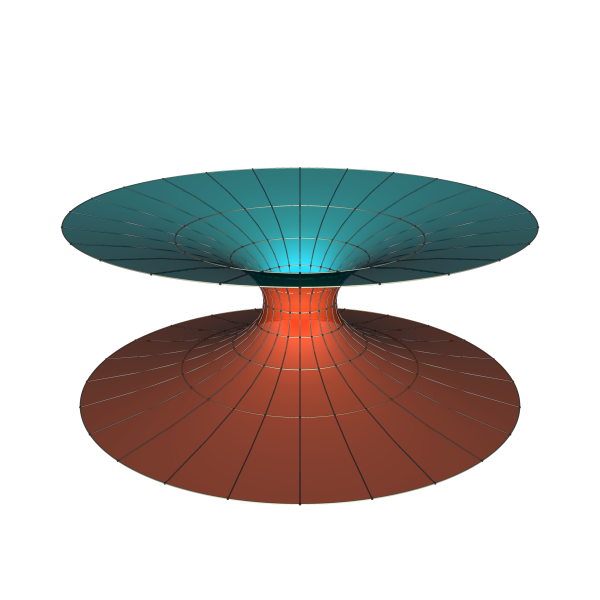
\includegraphics[width=0.5\textwidth]{images/catenoid}
%		\caption{Catenoide. Autor: Matthias Weber. Licencia: Creative Commons Attribution-Noncommercial-No Derivative Works 3.0 Unported License (\url{http://creativecommons.org/licenses/by-nc-nd/3.0/}). Enlace: \url{https://minimal.sitehost.iu.edu/archive/Classical/Classical/Catenoid/web/index.html}}
		\caption{Catenoide.}
	\end{figure}

\end{frame}

\begin{frame}

		\begin{exemplo}
		O \alert{helicoide} é uma superfície mínima em $\R^3$ parametrizada por
		\begin{equation*}
		\varphi(u,v) = \parentheses{a \sinh v \cos u, a \sinh v \sin u, au},
		\end{equation*}
		onde $u \in \parentheses{0, 2\pi}$ e $v \in \R$.
	\end{exemplo}
	Neste exemplo temos
	\begin{equation*}
	E = G = a^2 \cosh^2 v, \quad F = 0 \quad \text{e} \quad \Delta \varphi \equiv 0.
	\end{equation*}
	
\end{frame}

\begin{frame}
	
	\begin{figure}
		\centering
		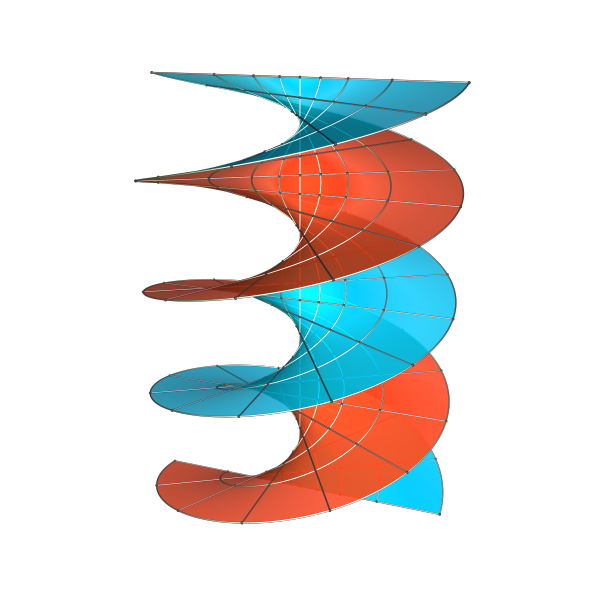
\includegraphics[width=0.5\textwidth]{images/helicoid}
%		\caption{Helicoide. Autor: Matthias Weber. Licencia: Creative Commons Attribution-Noncommercial-No Derivative Works 3.0 Unported License (\url{http://creativecommons.org/licenses/by-nc-nd/3.0/}). Enlace: \url{https://minimal.sitehost.iu.edu/archive/Classical/Classical/Helicoid/web/index.html}}
		\caption{Helicoide.}
	\end{figure}
\end{frame}

\begin{frame}
	\frametitle{Aplicação (Bolhas de sabão)}
	
	\begin{itemize}
		\item Os objetos matemáticos que modelam as bolhas de sabão são as superfícies em $\R^3$.
		\pause
		\item A energia potencial é proporcional a sua área superficial. (Gauss).
		\pause
		\item Pelo principio de Johann Bernoulli de trabalho virtual, as bolhas de sabão em estado de equilíbrio corresponde a superfícies de área mínima.
	\end{itemize}
	
%	Os objetos matemáticos que modelam os películas de sabão são as superfícies em $\R^3$. Para cada superfície, a teoria fenomenológica da capilaridade, devida a Gauss, afirma que a energia potencial é proporcional a sua área superficial. Assim, pelo principio de Johann Bernoulli de trabalho virtual, os filmes de sabão em estado de equilíbrio corresponde a superfícies de área mínima. \cite{Dierkes2010}.
	
\end{frame}

\begin{frame}	
	
	\begin{figure}
		\centering
		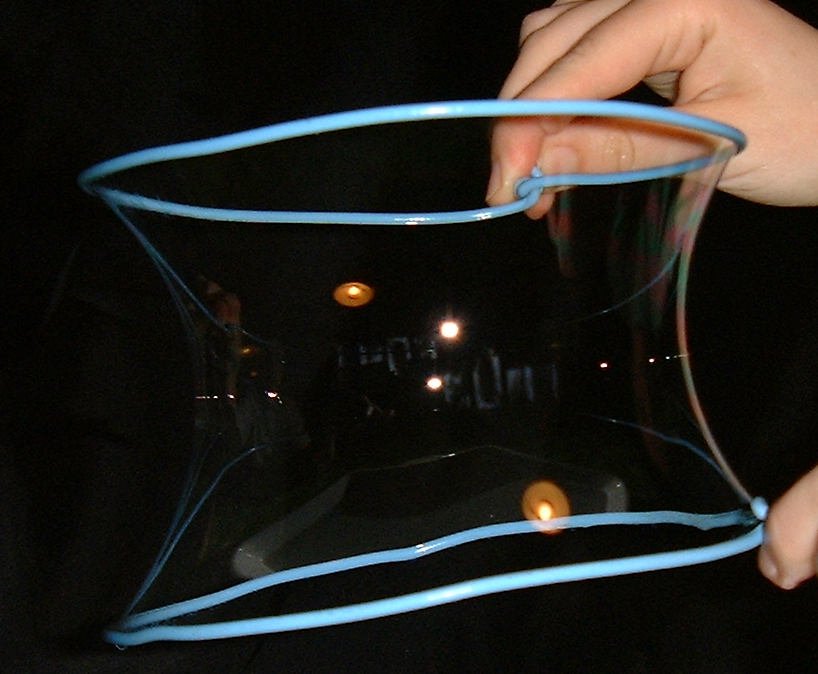
\includegraphics[width=0.5\textwidth]{images/soap-catenoid}
		%		\caption{Helicoide. Autor: Matthias Weber. Licencia: Creative Commons Attribution-Noncommercial-No Derivative Works 3.0 Unported License (\url{http://creativecommons.org/licenses/by-nc-nd/3.0/}). Enlace: \url{https://minimal.sitehost.iu.edu/archive/Classical/Classical/Helicoid/web/index.html}}
		\caption{Catenoide de sabão.}
	\end{figure}
	
\end{frame}

\begin{frame}
	\frametitle{Imersões isométricas}
	
	\begin{definicao}
		Dados duas variedades Riemannianas $M^m$ e $\tilde{M}^n$, uma \alert{imersão isométrica} entre $M$ e
		$\tilde{M}$ é uma aplicação diferenciável $f : M \rightarrow \tilde{M}$ que é uma imersão e, para todo $p \in M$, satisfaz
		\begin{equation*}
			\innerproduct{X}{Y} = \innerproduct{df(p) X}{df(p) Y},
		\end{equation*}
		para quaisquer $X,Y \in T_p M$.
	\end{definicao}

\end{frame}

\begin{frame}

	\begin{definicao}
		Dado uma imersão isométrica $f: M \rightarrow \tilde{M}$, seja $f^* T\tilde{M}$ o \alert{fibrado induzido} sobre $M$, cuja fibra em $p \in M$ é $T_{f(p)} \tilde{M}$. O complemento ortogonal de $f_* T_p M$ em $T_{f(p)} \tilde{M}$, denotado por $T_p M^\perp$, chama-se o \alert{espaço normal} de $f$ em $p$. O \alert{fibrado normal} $TM^\perp$ de $f$ é o subfibrado vetorial de $f^* T \tilde{M}$, cuja fibra em $p \in M$ é $T_p M^\perp$.  
	\end{definicao}

	\begin{itemize}
		\pause
		\item 	A conexão Levi-Civita $\tilde{\nabla}$ de $\tilde{M}$ induz uma única conexão $\hat{\nabla}$ em $f^* T \tilde{M}$ tal que
		\begin{equation*}
		\hat{\nabla}_X (Z \circ f) = \tilde{\nabla}_{f_* X} Z, 
		\end{equation*}
		para quaisquer $X \in \vectorfieldsspace{M}$ e $Z \in \vectorfieldsspace{\tilde{M}}$.
	\end{itemize}
	
\end{frame}

\begin{frame}

	\begin{itemize}
		\item Identificaremos sempre $\hat{\nabla}$ com $\tilde{\nabla}$.
		\pause
		\item 	Dados dois campos $X,Y \in \vectorfieldsspace{M}$, decompomos
		\begin{equation*}
		\tilde{\nabla}_X f_* Y = \parentheses{\tilde{\nabla}_X f_* Y}^\top + \parentheses{\tilde{\nabla}_X f_* Y}^\perp,
		\end{equation*}  
		em relação à descomposição ortogonal
		\begin{equation*}
		f^* T \tilde{M} = f_* TM \oplus TM^\perp.
		\end{equation*}
		\pause
		\item 	A aplicação
		\begin{equation*}
		\nabla_X Y = f_*^{-1} \parentheses{\tilde{\nabla}_X f_* Y}^\top
		\end{equation*}
		define uma conexão compatível e sem torção em $TM$, logo coincide com a conexão Levi-Civita de $M$.
	\end{itemize}
	
%	A conexão Levi-Civita $\tilde{\nabla}$ de $\tilde{M}$ induz uma única conexão $\hat{\nabla}$ em $f^* T \tilde{M}$ tal que
%	\begin{equation*}
%	\hat{\nabla}_X (Z \circ f) = \tilde{\nabla}_{f_* X} Z, 
%	\end{equation*}
%	para quaisquer $X \in \vectorfieldsspace{M}$ e $Z \in \vectorfieldsspace{\tilde{M}}$. Identificaremos sempre $\hat{\nabla}$ com $\tilde{\nabla}$.
%	
%	Dados dois campos $X,Y \in \vectorfieldsspace{M}$, decompomos
%	\begin{equation*}
%	\tilde{\nabla}_X f_* Y = \parentheses{\tilde{\nabla}_X f_* Y}^\top + \parentheses{\tilde{\nabla}_X f_* Y}^\perp,
%	\end{equation*}  
%	em relação à descomposição ortogonal
%	\begin{equation*}
%	f^* T \tilde{M} = f_* TM \oplus TM^\perp.
%	\end{equation*}
%	
%	A aplicação
%	\begin{equation*}
%	\nabla_X Y = f_*^{-1} \parentheses{\tilde{\nabla}_X f_* Y}^\top
%	\end{equation*}
%	define uma conexão compatível e sem torção em $TM$, logo coincide com a conexão Levi-Civita de $M$.

\end{frame}

\begin{frame}
	
	\begin{definicao}<1->
		A aplicação $\alpha_f: \vectorfieldsspace{M} \times \vectorfieldsspace{M} \rightarrow \Gamma(TM^\perp)$ definida por
		\begin{equation*}
		\alpha_f(X,Y) = \parentheses{\tilde{\nabla}_X f_* Y}^\perp,
		\end{equation*}
		chama-se de \alert{segunda forma fundamental} da imersão isométrica $f$.
	\end{definicao}
	
	\begin{teorema}<2->[Equação de Gauss]
		Para $X,Y,Z,W \in \vectorfieldsspace{M}$ quaisquer, cumpre-se a seguinte equação
		\begin{align*}
			\innerproduct{\tilde{R}(X,Y)Z}{W} &= \innerproduct{R(X,Y)Z}{W} - \innerproduct{\alpha_f(X,W)}{\alpha_f(Y,Z)}\\
			&+ \innerproduct{\alpha_f(X,Z)}{\alpha_f(Y,W)}.
		\end{align*}
		onde $\tilde{R}$ e $R$ são os endomorfismos de curvatura de $\tilde{M}$ e $M$ respectivamente.
	\end{teorema}

\end{frame}

\begin{frame}

	\begin{itemize}
		\item Para a imersão isométrica $f: M^2 \rightarrow \mathbb{Q}^3_c$, a curvatura seccional de $M^2$ coincide com sua curvatura intrínseca.
		\pause
		\item Portanto temos a seguente proposição:
		\pause
	\end{itemize}
	
%	Em particular, para a imersão isométrica $f: M^2 \rightarrow \mathbb{Q}^3_c$, onde $M^2$ é uma variedade Riemanniana de dimensão 2 e $\mathbb{Q}^3_c$ é uma forma espacial completa simplesmente conexa de curvatura seccional constante de dimensão 3, i.e, $\R^3$, $\Sp^3_c$ ou $\mathbb{H}^3_c$, a curvatura seccional de $M^2$ coincide com sua curvatura intrínseca. Portanto temos a seguente proposição:

	\begin{proposicao}
		A curvatura Gaussiana intrínseca $K_{\text{int}}$ de $M^2$ é dada por
		\begin{equation*}
			K_{\text{int}} = K_{\text{ext}} + c,
		\end{equation*}
		onde $K_{\text{ext}}$ denota a curvatura extrínseca de $M^2$, que é dada pelo produto das curvaturas principais de $M^2$.
	\end{proposicao}

	\pause

	\begin{itemize}
		\item Vamos agora a generalizar as definições de curvatura média e superfície mínima para imersões isométricas.
	\end{itemize}
	
\end{frame}

\begin{frame}

	\begin{definicao}
		O \alert{vetor curvatura média} de $f$ no ponto $p \in M$ é o vetor normal
		\begin{equation}\label{vetor-curvatura-media}
		H(p) = \frac{1}{m} \sum_{i=1}^m \alpha_f(X_i,X_i),
		\end{equation}
		onde $\{X_1, \ldots, X_m \}$ é uma base ortonormal de $T_p M$. Segue de \eqref{vetor-curvatura-media} que
		\begin{align*}
		m \innerproduct{H}{\xi} &= \sum_{i=1}^m \innerproduct{\alpha_f(X_i,X_i)}{\xi} = \sum_{i=1}^m \innerproduct{A_{\xi} X_i}{X_i}\\
		&= \tr A_{\xi},
		\end{align*}
		logo o lado direito de \eqref{vetor-curvatura-media} não depende da escolha da base ortonormal.
	\end{definicao}

\end{frame}

\begin{frame}

	\begin{definicao}
		Uma imersão isométrica $f: M \rightarrow \tilde{M}$ é dita ser \alert{mínima} no ponto $p \in M$ se $H(p)=0$. Diremos que $f$ é \alert{mínima} se for mínima em todos os pontos $p \in M$.
	\end{definicao}

	\pause

	\begin{observacao}
		La definição de superfícies mínimas em $\R^3$ é \alert{um caso particular} desta definição mais geral quando $M$ e $\tilde{M}$ são $\R^2$ e $\R^3$ respectivamente.
	\end{observacao}
\end{frame}


\begin{frame}
	\frametitle{Superfícies mínimas em $\Sp^3$}

	\begin{observacao}
		Enquanto que em $\R^3$ não existem superfícies mínimas compactas, em $\Sp^3$ temos exemplos.
	\end{observacao}

	\pause

	\begin{exemplo}
		A superfície compacta em $\Sp^3$ definida por
		\begin{equation*}
		M = \{ x \in \Sp^3 \subset \R^4: x_4 = 0 \},
		\end{equation*}
		é chamada de \alert{equador} e é uma superfície mínima porque ambas curvaturas principais são iguais a zero.
	\end{exemplo}

%	\pause
%	
%	\begin{itemize}
%		
%	\end{itemize}
	 
	
%	\begin{definicao}
%		Seja $f: \R^2 \rightarrow \Sp^3$ definida por
%		\begin{equation*}
%		f(u,v) = \frac{1}{\sqrt{2}} \left(\cos u, \sin u, \cos v, \sin v\right).
%		\end{equation*}
%		$f$ é chamada de \emph{toro de Clifford}.
%	\end{definicao}
%	
%	\begin{observacao}
%		$f$ é um toro porque é congruente com $\Sp^1 \left(\frac{1}{\sqrt{2}}\right) \times \Sp^1 \left(\frac{1}{\sqrt{2}}\right)$.
%	\end{observacao}
\end{frame}



\begin{frame}
	\frametitle{O toro de Clifford}
	
	\begin{itemize}
		\item Outro exemplo de uma superfície mínima compacta em $\Sp^3$ é o \alert{toro de Clifford}.
		
		\pause
		
		\item 	Seja a aplicação $x: \R^2 \rightarrow \R^4$ definida por
		\begin{equation}\label{def:toro-de-clifford}
		x(u,v) = \frac{1}{\sqrt{2}} \parentheses{\cos u, \sin u, \cos v, \sin v}.
		\end{equation}
		
		\pause
		
		\item $x$ é uma aplicação diferenciável e tem-se
		\[ \frac{\partial x}{\partial u} = \frac{1}{\sqrt{2}} \parentheses{-\sin u, \cos u, 0, 0} \]
		e
		\[ \frac{\partial x}{\partial v} = \frac{1}{\sqrt{2}} \parentheses{0,0, -\sin v, \cos v}. \]
		
		
	\end{itemize}

\end{frame}

\begin{frame}

	\begin{itemize}
		\item $x$ é uma imersão.
		
		\pause
	
		\item Como 
		\[x(u + 2k \pi, v + 2l \pi) = x(u,v), \] 
		para quaisquer $(u,v) \in \R^2$ e $k,l \in \mathbb{Z}$, segue que a imagem $x(\R^2)$ é um toro $\Sp_{\sqrt{2}}^1 \times \Sp_{\sqrt{2}}^1 \subset \R^4$.
		
		\pause
		
		\item Fixemos o referencial ortogonal:
		\begin{align*}
		e_1 &= \frac{\partial x}{\partial u},\\
		e_2 &= \frac{\partial x}{\partial v},\\
		e_3 &= \frac{1}{\sqrt{2}} \parentheses{\cos u, \sin u, \cos v, \sin v},\\
		e_4 &= \frac{1}{\sqrt{2}} \parentheses{-\cos u, -\sin u, \cos v, \sin v}.
		\end{align*}
		
	\end{itemize}

\end{frame}

\begin{frame}

	\begin{itemize}
		
		\item O vetor posição $e_3 = x$ descreve uma esfera unitária, pois $\norm{x} = 1$. Assim, o toro $x(\R^2)$ está contido na esfera unitária $\Sp^3 \subset \R^4$.
		
		\pause
		
		\item O referencial $\{e_1,e_2,e_4\}$ é tangente a $\Sp^3$, com
		$e_4$ normal ao toro $x(\R^2)$.
		
		\pause
		
		\item Como imersão isométrica, $x: \Sp_{\sqrt{2}}^1 \times \Sp_{\sqrt{2}}^1 \rightarrow \Sp^3$ é conhecida como o \alert{toro de Clifford}.
		
	\end{itemize}

\end{frame}

\begin{frame}

	\begin{itemize}
		
		\item Seja $(h_{ij})$ a matriz da segunda forma fundamental do toro em relação ao campo normal $e_4$. Cada entrada da matriz é dada por
		\begin{equation*}
		\begin{split}
		h_{11} &= \innerproduct{A e_1}{e_1}\\
		h_{12} &= \innerproduct{A e_1}{e_2}\\
		h_{21} &= \innerproduct{A e_2}{e_1}\\
		h_{22} &= \innerproduct{A e_2}{e_2}
		\end{split},
		\end{equation*}
		onde $AX$ é dado por
		\[ AX = -\tilde{\nabla}_X e_4, \]
		para qualquer vetor tangente $X$ ao toro $x(\R^2)$.
		
	\end{itemize}

\end{frame}

\begin{frame}

	\begin{itemize}
		
		\item Temos:
		\begin{align*}
		A e_1 &= -\tilde{\nabla}_{\frac{\partial}{\partial u}} e_4 = \frac{1}{\sqrt{2}} \parentheses{-\sin u, \cos u, 0, 0},\\
		A e_2 &= -\tilde{\nabla}_{\frac{\partial}{\partial v}} e_4 = \frac{1}{\sqrt{2}} \parentheses{0,0, \sin v, -\cos v}.
		\end{align*}
		
		\pause
		
		\item Substituindo, obtemos:
		\[ h_{11} = 1, \qquad h_{12}=h_{21}=0 \qquad \text{e} \qquad h_{22} = -1. \]
		
		\pause
		
		\item Disso decorre, em particular, que as curvaturas principais do toro $x(\R^2)$ são $\lambda_1 = 1$ e $\lambda_2 = -1$, ou seja, \alert{o toro de Clifford é uma superfície mínima}.
	\end{itemize}
	
%	Considere a aplicação $x: \R^2 \rightarrow \R^4$ definida por
%	\begin{equation}\label{def:toro-de-clifford}
%	x(u,v) = \frac{1}{\sqrt{2}} \parentheses{\cos u, \sin u, \cos v, \sin v}.
%	\end{equation}
%	Claramente $x$ é uma aplicação diferenciável e tem-se
%	\[ \frac{\partial x}{\partial u} = \frac{1}{\sqrt{2}} \parentheses{-\sin u, \cos u, 0, 0} \]
%	e
%	\[ \frac{\partial x}{\partial v} = \frac{1}{\sqrt{2}} \parentheses{0,0, -\sin v, \cos v}. \]
%	Disso decorre, em particular, que $x$ é uma imersão. Além disso, como 
%	\[x(u + 2k \pi, v + 2l \pi) = x(u,v), \] 
%	para quaisquer $(u,v) \in \R^2$ e $k,l \in \mathbb{Z}$, segue que a imagem $x(\R^2)$ é um toro $\Sp_{\sqrt{2}}^1 \times \Sp_{\sqrt{2}}^1 \subset \R^4$. A fim de entender a geometria deste toro, fixemos o seguinte referencial ortonormal:
%	\begin{align*}
%	e_1 &= \parentheses{-\sin u, \cos u, 0, 0},\\
%	e_2 &= \parentheses{0, 0, -\sin v, \cos v},\\
%	e_3 &= \frac{1}{\sqrt{2}} \parentheses{\cos u, \sin u, \cos v, \sin v},\\
%	e_4 &= \frac{1}{\sqrt{2}} \parentheses{-\cos u, -\sin u, \cos v, \sin v}.
%	\end{align*}
%	Observe que o vetor posição $e_3 = x$ descreve uma esfera unitária, pois $\norm{x} = 1$. Assim, o toro $x(\R^2)$ está contido na esfera unitária $\Sp^3 \subset \R^4$. Além disso, o referencial $\{e_1,e_2,e_4\}$ é tangente a $\Sp^3$, com
%	$e_4$ normal ao toro $x(\R^2)$. Como imersão isométrica, $x: \Sp_{\sqrt{2}}^1 \times \Sp_{\sqrt{2}}^1 \rightarrow \Sp^3$ é conhecida como o \emph{toro de Clifford}. Denotemos por $(h_{ij})$ a matriz da segunda forma fundamental do toro em relação ao campo normal $e_4$. Cada entrada da matriz é dada por
%	\begin{equation*}
%	\begin{split}
%	h_{11} &= \innerproduct{A e_1}{e_1}\\
%	h_{12} &= \innerproduct{A e_1}{e_2}\\
%	h_{21} &= \innerproduct{A e_2}{e_1}\\
%	h_{22} &= \innerproduct{A e_2}{e_2}
%	\end{split},
%	\end{equation*}
%	onde $AX$ é dado por
%	\[ AX = -\tilde{\nabla}_X e_4, \]
%	para qualquer vetor tangente $X$ ao toro $x(\R^2)$. Temos:
%	\begin{align*}
%	A e_1 &= -\tilde{\nabla}_{\frac{\partial}{\partial u}} e_4 = \frac{1}{\sqrt{2}} \parentheses{-\sin u, \cos u, 0, 0},\\
%	A e_2 &= -\tilde{\nabla}_{\frac{\partial}{\partial v}} e_4 = \frac{1}{\sqrt{2}} \parentheses{0,0, \sin v, -\cos v}.
%	\end{align*}
%	Substituindo, obtemos:
%	\[ h_{11} = \frac{1}{\sqrt{2}}, \qquad h_{12}=h_{21}=0 \qquad \text{e} \qquad h_{22} = -\frac{1}{\sqrt{2}}. \]
%	Disso decorre, em particular, que as curvaturas principais do toro $x(\R^2)$ são $\lambda_1 = \frac{1}{\sqrt{2}}$ e $\lambda_2 = -\frac{1}{\sqrt{2}}$, ou seja, o toro de Clifford é uma superfície mínima.
\end{frame}

\begin{frame}
	
	
	\begin{observacao}
		Por muito tempo o equador e o toro de Clifford eram os únicos exemplos de superfícies mínimas mergulhadas em $\Sp^3$. No entanto, isso mudou fortemente no final dos
		anos 1960 quando Blaine Lawson descobriu uma família infinita de superfícies mínimas
		mergulhadas em $\Sp^3$ de genus arbitrário \cite{Lawson1970}.
	\end{observacao}
	
	\pause
	
	\begin{teorema}[\cite{Lawson1970}]
		Existe ao menos uma superfície mínima mergulhada em $\Sp^3$	de gênero $g$, onde $g$ é um inteiro não negativo. Se $g$ não for primo, o mergulho não é único.
	\end{teorema}
	
	\pause
	
	\begin{observacao}
		A questão de unicidade para superfícies mínimas mergulhadas na esfera $\Sp^3$ com genus $0$ foi provada por Algrem \cite{Almgren1966}.
	\end{observacao}
\end{frame}


\section{Conjectura de Lawson}

\begin{frame}
	\frametitle{Conjectura de Lawson}
	

	\begin{observacao}
		A hipótese de ser mergulhada é fundamental. De fato, em \cite{Lawson1969}, Lawson construiu uma família (infinita) de imersões mínimas de toros em $\Sp^3$. 
	\end{observacao}

	\pause

	\begin{proposicao}[\cite{Brendle2013}]
		\label{sup-min-nao-tem-pontos-umbilicos}
		Uma superfície mínima imersa em $\Sp^3$ de genus 1 não tem pontos umbílicos, i.e., a segunda forma fundamental não é zero em tudo ponto da superfície.
	\end{proposicao}

\end{frame}

\begin{frame}

	\begin{itemize}
		\item Seja $\Psi: \Sigma \rightarrow \R$ tal que
		\begin{equation*}
		\Psi(x) = \frac{\norm{A(x)}}{\sqrt{2}},
		\end{equation*}
		onde $A$ é a segunda forma fundamental.
	\end{itemize}
	
	\pause
	
	\begin{observacao}
		Pela Proposição \ref{sup-min-nao-tem-pontos-umbilicos}, $\Psi(x) \neq 0$.
	\end{observacao}

	\pause

	\begin{definicao}
		Uma imersão $f: M \rightarrow \overline{M}$ é \alert{geodésica} em $p \in M$ se para todo $\eta \in \parentheses{T_p M}^\perp$ a segunda forma fundamental $A_\eta$ é identicamente nula em $p$. A imersão é \alert{totalmente geodésica} se ela é geodésica para todo $p \in M$.
	\end{definicao}

\end{frame}

\begin{frame}

	\begin{teorema}[\cite{Lawson1969}]
		\label{curv-gauss-de-sup-min-em-S3}
		Se $M^2$ é uma superfície mínima em $\Sp^3$ de curvatura Gaussiana constante $K$, então $K=1$ e $M^2$ é totalmente geodésica, ou $K=0$ e $M^2$ é um pedaço aberto do toro de Clifford.
	\end{teorema}

	\pause

	\begin{proposicao}\label{aleph-leq-1}
		Se
		\begin{equation*}
		\sup_{\substack{x,y \in \Sigma \\ x \neq y}} \frac{\norm{\innerproduct{\nu(x)}{F(y)}}}{\Psi(x) (1-\innerproduct{F(x)}{F(y)})} \leq 1,
		\end{equation*}
		então $F$ é congruente ao toro de Clifford.
	\end{proposicao}

\end{frame}

\begin{frame}

	\begin{itemize}
		\item Da desigualdade do enunciado, temos que
		\begin{equation*}
		\Psi(x) (1-\innerproduct{F(x)}{F(y)}) + \innerproduct{\nu(x)}{F(y)} \geq 0.
		\end{equation*}
		
		\pause
		
		\item Seja $\{ e_1,e_2 \}$ uma base ortonormal de $T_x \Sigma$ tal que
		\begin{equation*}
		h(e_1,e_1)=\Psi(x), \quad h(e_1,e_2)=0 \quad e \quad h(e_2,e_2)=-\Psi(x)
		\end{equation*}
		
		\pause
		
		\item Identificando $F(x)$ com $x$, seja $\gamma$ uma geodésica tal que $\gamma(0)=x$ e $\gamma'(0)=e_1$.
		
		\pause
		
		\item Definamos a função $f: \R \rightarrow \R$ tal que
		\begin{equation*}
		f(t) = \Psi(x) (1-\innerproduct{x}{\gamma(t)}) + \innerproduct{\nu(x)}{\gamma(t)} \geq 0.
		\end{equation*}
	
	\end{itemize}

\end{frame}

\begin{frame}

	\begin{itemize}

		\item Calculando as derivadas de $f$ tem-se:
		\begin{align*}
		f'(t) =& -\innerproduct{\Psi(x)x - \nu(x)}{\gamma'(t)},\\
		f''(t) =& \innerproduct{\Psi(x)x - \nu(x)}{\gamma(t)}\\
		& + h(\gamma'(t),\gamma'(t)) \innerproduct{\Psi(x)x - \nu(x)}{\nu(\gamma(t))},\\
		f'''(t) =& \innerproduct{\Psi(x)x - \nu(x)}{\gamma'(t)}\\
		& + h(\gamma'(t),\gamma'(t)) \innerproduct{\Psi(x)x - \nu(x)}{D_{\gamma'(t)} \nu(\gamma(t))}\\
		& + (D_{\gamma'(t)} h) (\gamma'(t),\gamma'(t)) \innerproduct{\Psi(x)x - \nu(x)}{\nu(\gamma'(t))}.
		\end{align*}
	
		\pause
		
		\item Avaliando em $0$ temos: $f(0)=f'(0)=f''(0)=0$.
		
		\pause
		
		\item Como $f(t) \geq 0$, então $f'''(0)=0$.
		
		\pause
		
		\item Portanto, $(D_{e_1}h)(e_1,e_1)=0$.
		
	\end{itemize}

\end{frame}

\begin{frame}

	\begin{itemize}	
		
		\item Mudando a orientação à base $\{ e_2, e_1, -\nu \}$, e procedendo de maneira similar, temos que $\parentheses{D_{e_2}h} \parentheses{e_2,e_2}=0$.
		
		\pause
		
		\item Usando as equações de Codazzi, podemos concluir que $\nabla h \equiv 0$.
		
		\pause
		
		\item Portanto, $h$ é constante, e com isso, a curvatura Gaussiana $K$ é constante.

		\pause

		\item Pelo Teorema \ref{curv-gauss-de-sup-min-em-S3}, a curvatura Gaussiana é $K \equiv 1$ ou $K \equiv 0$.
		
		\pause
		
		\item Se $K=1$, então $F$ tem pontos umbílicos. 
		Isso é uma contradição.
		
		\pause
		
		\item Portanto a curvatura Gaussiana $K \equiv 0$ e $F$ é um pedaço aberto do toro de Clifford.
		Como $F$ é compacta, então $F$ é o toro de Clifford.
		\qed
	\end{itemize}

\end{frame}

\begin{frame}
	
	\begin{itemize}
		\item Definamos $\aleph$ da seguinte forma:
		\begin{equation*}
		\aleph = \sup_{\substack{x,y \in \Sigma \\ x \neq y}} \frac{\norm{\innerproduct{\nu(x)}{F(y)}}}{\Psi(x) (1-\innerproduct{F(x)}{F(y)})}.
		\end{equation*}
	\end{itemize}
	
	\pause
	
	\begin{observacao}
		Pela Proposição \ref{aleph-leq-1}, quando $\aleph \leq 1$ temos que a superfície é o toro de Clifford. 
	\end{observacao}

	\pause

	\begin{itemize}
		\item A partir de agora vamos analisar o caso onde $\aleph > 1$.
		
		\pause
		
		\item 	Da definição de $\aleph$, podemos ter a função $Z: \Sigma \times \Sigma \rightarrow \R$ descrita da forma:
		\begin{equation*}
		Z(x,y) = \aleph \Psi(x) \left(1 - \innerproduct{F(x)}{F(y)} \right) + \innerproduct{\nu(x)}{F(y)}.
		\end{equation*}
		
		
	\end{itemize}

\end{frame}
	
\begin{frame}

	\begin{itemize}
		\item $Z(x,y) \geq 0$ para todo $x,y \in \Sigma$.
		
		\pause
		
		\item Sejam $(x_1,x_2)$ coordenadas normais geodésicas ao redor de $x$ e $(y_1,y_2)$ coordenadas normais geodésicas ao redor de $y$.
		
		\pause
		
		\item A derivada de $Z$ com respeito a $x_i$ está dado por
		\begin{multline*}
		\partialdiff{Z}{x_i}(x,y) = \aleph \partialdiff{\Psi}{x_i}(x) \parentheses{1 - \innerproduct{F(x)}{F(y)}} \\
		-\aleph \Psi(x) \innerproduct{\partialdiff{F}{x_i}(x)}{F(y)} + \sum_{k=1}^{2} h_{ik}(x) \innerproduct{\partialdiff{F}{x_k}(x)}{F(y)}.
		\end{multline*}
		
		\pause
		
		\item A derivada de $Z$ com respeito a $y_i$ está dado por
		\begin{equation*}
		\frac{\partial Z}{\partial y_i}(x,y) = -\aleph \Psi(x) \innerproduct{F(x)}{\frac{\partial F}{\partial y_i}(y)} + \innerproduct{\nu(x)}{\frac{\partial Z}{\partial y_i}(y)}.
		\end{equation*}
	\end{itemize}
	
\end{frame}
	
\begin{frame}



	\begin{proposicao}\label{sum-2nd-derivative-z-inequality}
		A função $Z$ cumpre a seguinte desigualdade:
		\begin{multline*}
			\sum_{i=1}^{2} \frac{\partial^2 Z}{\partial x_i^2}(x,y) + 2 \sum_{i=1}^{2} \frac{\partial^2 Z}{\partial x_i \partial y_i}(x,y) + \sum_{i=1}^{2} \frac{\partial^2 Z}{\partial y_i^2}(x,y) \leq \\
			- \frac{\aleph^2 -1}{\aleph} \frac{\Psi(x)}{1 - \innerproduct{F(x)}{F(y)}} \sum_{i=1}^{2} \innerproduct{\frac{\partial F}{\partial x_i}(x)}{F(y)}^2 \\ 
			+ \overline{\Lambda}(x,y) \left( Z(x,y) + \sum_{i=1}^{2} \left| \frac{\partial Z}{\partial x_i}(x,y) \right| + \sum_{i=1}^{2} \left| \frac{\partial Z}{\partial y_i}(x,y) \right| \right),
		\end{multline*}
		onde $\overline{\Lambda}(x,y)$ é contínua e pode não ser limitada em uma vizinhança da diagonal.
	\end{proposicao}

\end{frame}

\begin{frame}

	\begin{teorema}[Principio do máximo estrito de Bony]
		\label{bony's-strict-maximum-principe}
		Seja $W$ um subconjunto aberto de $\R^n$, e sejam $X_1, \ldots, X_m$ campos vetoriais diferenciais em $W$. Assuma que $\varphi: W \rightarrow \R$ é uma função diferenciável não negativa satisfazendo
		\begin{equation*}
			\sum_{j=1}^{m} D^2 \varphi (X_j,X_j) \leq -L \inf_{|\xi| \leq 1} D^2 \varphi(\xi,\xi) + L \varphi + L |D \varphi|,
		\end{equation*}
		onde $L$ é uma constante positiva. Seja $F= \{ x \in W: \varphi(x)=0 \}$ o conjunto de zeros da função $\varphi$. Adicionalmente, suponha que $\gamma: [0,1] \rightarrow W$ é um caminho diferenciável tal que $\gamma(0) \in F$ e $\gamma'(s) = \sum_{j=1}^{m} f_j(s) X_j(\gamma(s))$ para funções diferenciáveis $f_1, \ldots, f_m: [0,1] \rightarrow \R$. Então $\gamma(s) \in F$ para tudo $s \in [0,1]$.
	\end{teorema}

\end{frame}

\begin{frame}


	\begin{observacao}
		O Teorema \ref{bony's-strict-maximum-principe} é válido ainda quando $W$ é um aberto de uma variedade Riemanniana. 
	\end{observacao}

	\pause

	\begin{itemize}
		\item Definamos o conjunto
		\begin{equation*}
		\Omega = \left\{ x \in \Sigma: \exists y \in \Sigma \setminus \{ x \}, Z(x,y)=0 \right\}.
		\end{equation*}
	\end{itemize}

	\pause
	
	\begin{proposicao}
		$\Omega$ não é vazio.
	\end{proposicao}

	\pause
	
	\begin{itemize}
		\item Como $\Psi(x) \parentheses{1 - \innerproduct{F(x)}{F(y)}}$ é contínua para $x,y \in \Sigma$ e $\Sigma$ é compacto, então existe $M>0$ tal que
		\begin{equation*}
			\Psi(x) \parentheses{1 - \innerproduct{F(x)}{F(y)}} \leq M.
		\end{equation*}
		
	\end{itemize}	
		
\end{frame}

\begin{frame}
		
	\begin{itemize}
		\item Pela definição de $\aleph$, tem-se que para qualquer $n \in \mathbb{N}$ existem $x_n,y_n \in \Sigma$, onde $x_n \neq y_n$, tal que
		\begin{equation*}
			\frac{- \innerproduct{\nu(x_n)}{F(y_n)}}{\Psi(x_n) \parentheses{1 - \innerproduct{F(x_n)}{F(y_n)}}} > \aleph - \frac{1}{nM}
		\end{equation*}
		
		\pause
		
		\item Logo tem-se
		\begin{equation*}
			\frac{1}{n} \geq \frac{\Psi(x_n) \parentheses{1 - \innerproduct{F(x_n)}{F(y_n)}}}{nM} > Z(x_n, y_n) \geq 0.
		\end{equation*}
		
		\pause
		
		\item Como $(x_n)$ e $(y_n)$ são sequências limitadas, então existem subsequências convergentes $(x_{n_k})$ e $(y_{n_k})$ tal que $x_{n_k} \rightarrow \xb$ e $y_{n_k} \rightarrow \yb$ onde $\xb,\yb \in \Sigma$.
	\end{itemize}

\end{frame}

\begin{frame}
	\begin{itemize}
		\item Considerando a subsequências e tomando limite, tem-se
		\begin{equation*}
			Z(\xb,\yb) = 0
		\end{equation*}
		
		\pause
		
		\item Se $\xb = \yb$ chega-se a uma contradição.
		
		\pause
		
		\item Portanto, $\xb \neq \yb$ e logo $\xb \in \Omega$.
	\end{itemize}

	\pause

	\begin{proposicao}
		$\Omega$ é aberto.
	\end{proposicao}

	\pause

	\begin{itemize}
		\item Para provar que $\Omega$ é aberto usa-se o Teorema \ref{bony's-strict-maximum-principe}.
	\end{itemize}

\end{frame}

\begin{frame}

	\begin{itemize}
		\item Em $\Omega$ temos que
		\begin{equation*}
		Z(x,y) + \sum_{i=1}^{2} \left| \frac{\partial Z}{\partial x_i}(x,y) \right| + \sum_{i=1}^{2} \left| \frac{\partial Z}{\partial y_i}(x,y) \right| = 0
		\end{equation*}
		
		\pause
		
		\item Logo, em $\Omega$, a Proposição \ref{sum-2nd-derivative-z-inequality} fica expressada
		\begin{align*}
		0 \leq \sum_{i=1}^{2} \frac{\partial^2 Z}{\partial x_i^2}(x,y) + 2 \sum_{i=1}^{2} \frac{\partial^2 Z}{\partial x_i \partial y_i}(x,y) + \sum_{i=1}^{2} \frac{\partial^2 Z}{\partial y_i^2}(x,y) \leq \\
		- \frac{\aleph^2 -1}{\aleph} \frac{\Psi(x)}{1 - \innerproduct{F(x)}{F(y)}} \sum_{i=1}^{2} \innerproduct{\frac{\partial F}{\partial x_i}(x)}{F(y)}^2 \leq 0,
		\end{align*}
		
		\pause
		
		\item A segunda derivada é definida não negativa porque $Z$ atinge seu mínimo em $(x,y)$.
	\end{itemize}

\end{frame}

\begin{frame}

	\begin{itemize}
		\item Portanto, 
		\begin{equation*}
		\innerproduct{\frac{\partial F}{\partial x_i}(x)}{F(y)} = 0,
		\end{equation*}
		para $i \in \{1;2\}$.
		
		\pause
		
		\item Usando a igualdade anterior e, sabendo que $\partialdiff{Z}{x_i}(x,y)=0$ em $\Omega$, $\partialdiff{Z}{x_i}(x,y)$ fica expressado por
		\begin{equation*}
		0 = \partialdiff{Z}{x_i}(x,y) = \aleph \partialdiff{\Psi}{x_i}(x) \parentheses{1 - \innerproduct{F(x)}{F(y)}}.
		\end{equation*}
		
		\pause
		
		\item Do anterior, conclui-se que
		\begin{equation*}
		\nabla \Psi(x) = 0, \quad \forall x \in \Omega.
		\end{equation*}
	\end{itemize}

\end{frame}	
	
\begin{frame}	

	\begin{itemize}
		\item Em particular,
		\begin{equation*}
		\Delta_{\Sigma} \Psi(x) = 0.
		\end{equation*}
	\end{itemize}	
	
	\pause

	\begin{proposicao}
		Seja $F: \Sigma \rightarrow \Sp^3$ um toro mínimo mergulhado em $\Sp^3$. A função $\Psi$ satisfaz a EDP
		\begin{equation*}
			\Delta_{\Sigma} \Psi - \frac{\norm{\nabla \Psi}^2}{\Psi} + \parentheses{\norm{A}^2 - 2} \Psi = 0.
		\end{equation*}
	\end{proposicao}

	\pause
	
	\begin{itemize}
		\item Da Proposição anterior,
		\[ \Psi(x) = 1, \quad \forall x \in \Omega. \]
	\end{itemize}

\end{frame}
	
\begin{frame}	
	
	\begin{itemize}
		\item Usando o teorema de extensão única para soluções de EDP elípticas (cf. \cite{Aronszajn1957}), concluímos que
		\[ \Psi(x) = 1, \quad \forall x \in \Sigma. \]
		
		\pause
		
		\item Conclui-se que
		\[ \lambda_1 = 1 \quad \text{e} \quad \lambda_2 = -1, \]
		onde $\lambda_1,\lambda_2$ são as curvaturas principais da superfície.
		
		\pause
		
		\item 	Portanto, a curvatura Gaussiana $K \equiv 0$ em $\Sigma$. Pelo Teorema \ref{curv-gauss-de-sup-min-em-S3}, $F$ é o toro de Clifford.
	\end{itemize}
	
	
	
	


\end{frame}

\begin{frame}
	\begin{center}
		\huge Obrigado pela atenção.
	\end{center}
\end{frame}

\begin{frame}[allowframebreaks]
	\frametitle{Referências}
	\bibliography{references}
\end{frame}

\end{document}